% Session 8 -- geometric frustration: the degenerate Ising triangle and the kagome lattice.
% Placement: sec. "Frustration: the route to a quantum spin liquid", after the
% triangular-plaquette paragraph.
% Rendered by figures/blender/s08f02_frustration.py, labels in figures/overlays/s08f02_frustration.tex.
\begin{aqmfigure}{fig:s08:frustration}{Frustration, with the spins drawn as Ising (collinear)
variables, which is how the argument in the text is written. If the spins can rotate freely, the
triangle goes instead into the $120^\circ$ noncollinear state of figure~\ref{fig:s06:frustration},
and the degeneracy that we discuss here is the Ising one. The plaquette without frustration and the
single frustrated triangle are panels (a) and (b) of figure~\ref{fig:s06:frustration}. On a
bipartite plaquette every antiferromagnetic bond can be satisfied at the same time, and the ground
state is the N\'eel state, with two configurations related by a global flip, each of which breaks
time-reversal symmetry. On a triangle this is not possible, since once two spins are antiparallel
the third bond cannot be satisfied for both directions of the last spin. (a) The frustrated bond, in
red, can be on any of the three edges, so the classical ground state is degenerate and not unique.
Quantum fluctuations mix the degenerate configurations into one superposition with $\langle\mathbf
S_i\rangle=\mathbf 0$, which does \emph{not} break time-reversal symmetry. (b) The kagome lattice of
herbertsmithite is built only from corner-sharing triangles, so all of them are frustrated at the
same time, here with one frustrated bond on every triangle, and the classical degeneracy becomes
macroscopic. This is why triangular and kagome lattices are the standard place to look for quantum
spin liquids.}
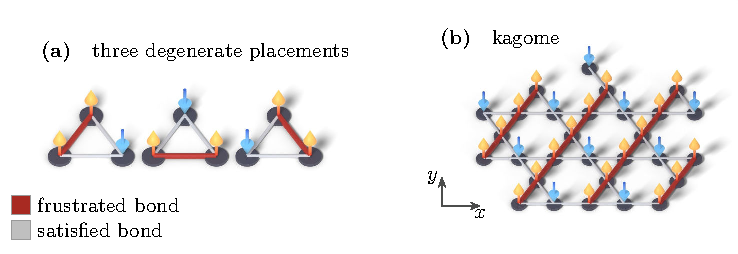
\includegraphics{figures/pdf/s08f02_frustration.pdf}
\end{aqmfigure}
